\documentclass[mathserif]{beamer}
%\usepackage[T1]{fontenc}
\mode<presentation> 
\usetheme{Warsaw}
\useinnertheme{rectangles}
\useoutertheme{infolines}
% centaur logo color: 174,191,219
\usecolortheme[RGB={134,151,179}]{structure}
\definecolor{Highlight}{rgb}{0,0,1}
\newcommand{\Highlight}[1]{{\color{Highlight}#1}}
\logo{
\includegraphics[scale=0.31]{logo}} 
\usepackage{comment}

\beamertemplatenavigationsymbolsempty

\newcommand{\ctxs}{\ensuremath{\textsc{CtxSize}}}

\usebeamerfont{title}
\usebeamerfont{author}
\usebeamerfont{institute}
\usebeamerfont{date}
\title{A Verilog Translator in ACL2}
\author[Page \thepage]{Jared Davis}
\institute{Centaur Technology}
\date{February 18, 2009}
\setlength{\parindent}{0pt}
\newcommand{\SmallSkip}{\vspace{0.5cm}\noindent}
\newcommand{\Skip}{\vspace{1cm}\noindent}
\newcommand{\MedSkip}{\vspace{1.5cm}\noindent}
\newcommand{\BigSkip}{\vspace{2cm}\noindent}
\begin{document}
\maketitle
\logo{}



\section[Introduction]{Introduction}
\begin{frame}
\frametitle{Introduction}

Previously --- a preprocessor, lexer, and parser for Verilog 2005, mostly in
logic mode with verified guards
\begin{itemize}
\item Simplicity over performance (1.5 mins., 10 GB memory)
\item Elaborate well-formedness checks, unit testing
\end{itemize}

\bigskip

Today --- a translator to convert the resulting parse tree into E modules

\bigskip

Think \Highlight{Verilog Simplifier} $\Highlight{+}$ \Highlight{Paren Transposer}
\begin{itemize}
\item We stay in Verilog as long as possible, rewriting modules into
 occurrence-based, register-transfer level descriptions
\item We want to produce a \Highlight{conservative approximation} of the input 
 modules w.r.t. the semantics of Verilog
\end{itemize}

\end{frame}


\begin{frame}
\begin{center}
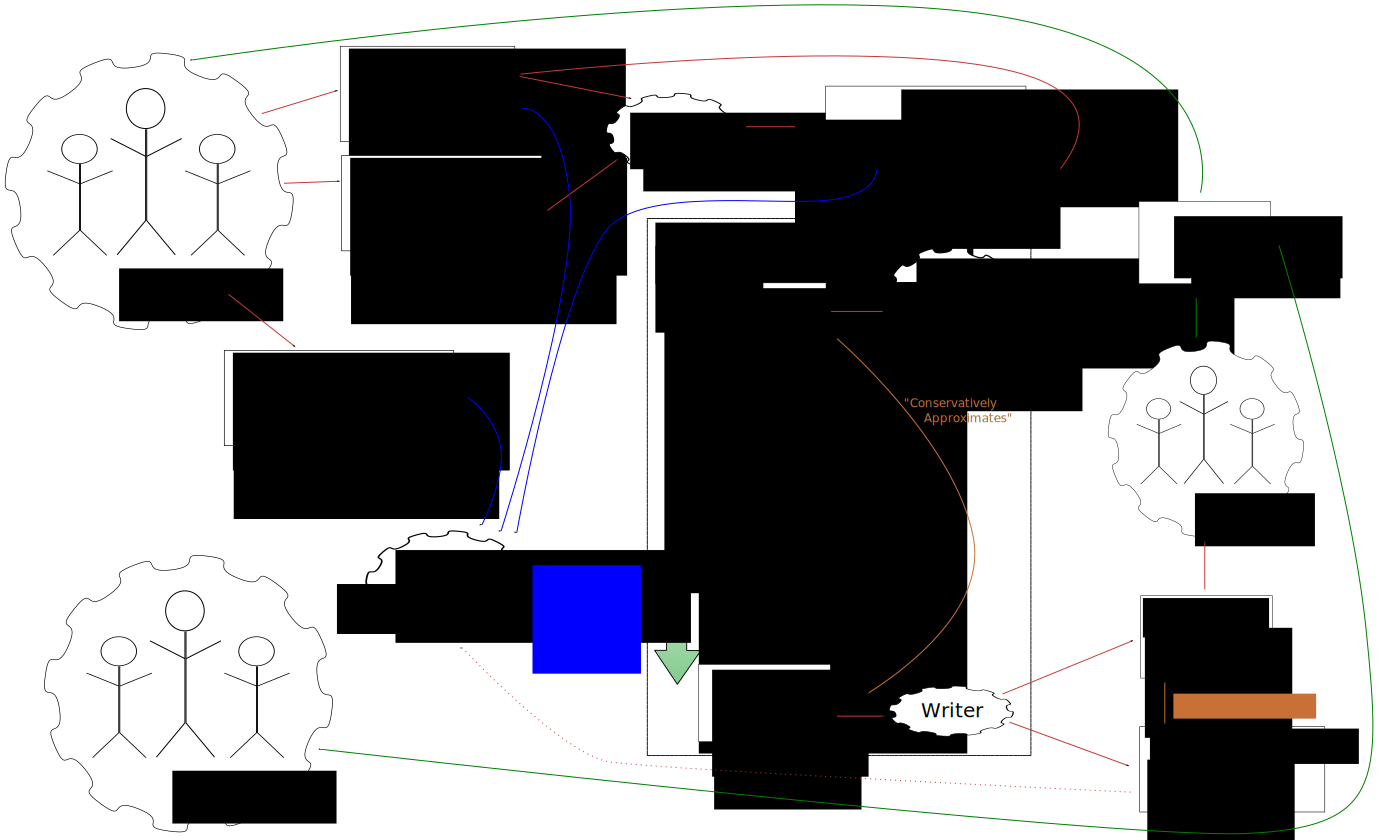
\includegraphics[width=12cm]{vl}
\end{center}
\end{frame}


\begin{frame}{Outline}
  \tableofcontents
\end{frame}




\section[Verilog semantics]{Verilog semantics}


\begin{frame}
\frametitle{Verilog semantics --- modules}

Modules are the basic building blocks of Verilog designs
\begin{itemize}
\item They have an interface of input and output ports
\item They may contain gates, registers, and instances of other modules
\end{itemize}

\bigskip

\begin{center}
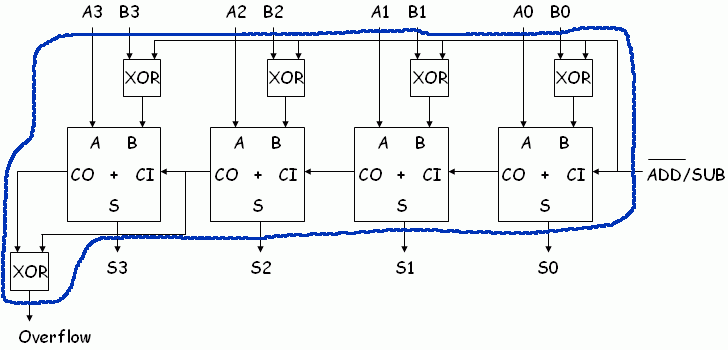
\includegraphics[scale=0.4]{adder_subtractor.png}
\end{center}

\end{frame}





\begin{frame}
\frametitle{Verilog semantics --- bits}

We consider only register-transfer level stuff (not transistor-level stuff)

\bigskip

Bits (on wires, in registers) can have four values
\begin{itemize}
\item 0 --- logical false (low)
\item 1 --- logical true (high)
\item X --- an unknown value
\item Z --- a high-impedance value (undriven)
\end{itemize}

\bigskip

Gate semantics are described in terms of these values with truth tables

{\small
\begin{center}
\begin{tabular}{ccc}
{\bf buf}  & & {\bf not} \\
\begin{tabular}{cc}
{\bf input} & {\bf output} \\
\hline
0 & 0 \\
1 & 1 \\
X & X \\
Z & X \\
\end{tabular} & \qquad \qquad &
\begin{tabular}{cc}
{\bf input} & {\bf output} \\
\hline
0 & 1 \\
1 & 0 \\
X & X \\
Z & X \\
\end{tabular}
\end{tabular}
\end{center}
}
\end{frame}


\begin{frame}
\frametitle{Verilog semantics --- vectors}

A wire/register can have a {\em range}, making it a vector of bits
\begin{itemize}
\item \texttt{wire [3:0] w;}
\end{itemize}

\bigskip

Such vectors can be interpreted in various ways
\begin{itemize}
\item Unsigned n-bit integers
\item Signed n-bit integers
\item ``Real'' numbers
\item Strings, times, and realtimes
\end{itemize}

\bigskip

We deal almost exclusively with unsigned integers
\begin{itemize}
\item 4'b 0011, 4'd 10, 8'h FF, 2'b XX
\end{itemize}

\bigskip




\end{frame}


\begin{frame}
\frametitle{Verilog semantics --- expressions}

Expressions can be used to concisely describe collections of gates
\begin{itemize}
\item \texttt{assign w = $\sim$(a \& b) $\hat{}$ (c + 4'b0010) ;}
\end{itemize}

\bigskip

A complex set of rules are used to determine how wide each operation is
\begin{itemize}
\item Does \texttt{c + 4'b0010}, above, produce a carry?
\end{itemize}

\bigskip

The semantics are described w.r.t. the 4-valued logic
\begin{itemize}
\item \texttt{a \& b} ands its arguments, bitwise, using the truth table for and
\item \texttt{a + b} produces X if any bit of either argument is X or Z
\item \texttt{a~?~b~:~c} combines \texttt{b} and \texttt{c} bit-by-bit when \texttt{a} is X or Z
\end{itemize}

\end{frame}



\begin{frame}[fragile]
\frametitle{Verilog semantics --- simulations}

Verilog is simultaneously
\begin{itemize}
\item A language for \Highlight{describing} circuits, and
\item A language for \Highlight{simulating} circuits over time
\end{itemize}

{\small
\begin{verbatim}
module test () ;
  reg a, b;
  wire o;
  and (o, a, b);

  initial
  begin
     a <= 0 ;
     b <= 1 ;
     $display("at time 0, o is %b", o);
     #1
     $display("at time 1, o is %b", o);
  end
endmodule
\end{verbatim}}
\bigskip

Updates happen and the time moves forward

\end{frame}

\begin{frame}
\frametitle{Conservative approximation}

Spec: every simplified module $M'$ should \Highlight{conservatively approximate} the input module, $M$

\bigskip

Roughly, and too ambitiously,

\begin{itemize}
\item $M'$ should have the same ports and internal state as $M$
\item $M'$ should have an instance of $S'$ whenever $M$ has an instance of $S$.
\item For every port and internal value, $M_p$, at every time $t$ of every simulation $s$, 
       $M'_p$ bit-approximates $M_p$,
\end{itemize}

Where ``bit-approximates'' means $M'_p = M_p$ or $M'_p$ is X

\bigskip

The approximation must be close enough to facilitate verification (i.e., all X's is not useful)
\end{frame}


\begin{frame}
\frametitle{The clock assumption}

Certain ports are known to be \Highlight{clocks}.

\bigskip

We assume there is enough time to update all other signals before any clock changes.

\bigskip

This is a huge assumption that rules out many Verilog simulations


\end{frame}


\begin{frame}
\frametitle{Verilog constructs that break conservativity}

Some Verilog constructs are broken w.r.t. conservativity
\begin{itemize}
\item {\tt if} treats X/Z as false
\item {\tt ===} and {\tt !==} treat X,Z as knowns
\item user-defined primitives may implement any X/Z behavior they like
\end{itemize}

\bigskip

We would eventually like to move away from using these constructs.

\bigskip
For now, we don't permit UDP's, and unsoundly
\begin{itemize}
\item Replace {\tt if} as the ternary operator, ?:
\item Treat {\tt ===} and {\tt !==} as {\tt ==} and {\tt !=}
\end{itemize}



\end{frame}



\section[Parse trees]{Parse trees}

\begin{frame}
\frametitle{Parse Trees}

Our parser produces a \Highlight{vl-modulelist-p} object, which is a list of
\Highlight{vl-module-p}'s.  Each of which has
\begin{itemize}
\item Name, ports
\item Parameter declarations
\item Port, register, variable, event, and wire declarations
\item Gate instances (occurrences)
\item Submodule instances (occurrences)
\item Continuous assignments
\item Always and initial statements
\end{itemize}

\bigskip
Most of these are compound structures.  Defaggregate, deflist.
\end{frame}

\begin{frame}
\frametitle{Basic module utilities}

We develop a number of utilities for working with modules
\begin{itemize}
\item Accessor projections (defprojection)
\item Modalists, module lookups
\item Modnamespaces, item lookups
\item Top-level/missing modules
\item Dependent/necessary modules
\item Dependency-order sorting
\item Pruning modules w.r.t. a keep-list
\end{itemize}

\bigskip
Fun stuff.  Logic mode, various theorems.  Lots of MBE.  Lots of Osets.
Could prove lots more.

\end{frame}


\begin{frame}
\frametitle{Reasonableness}

A module is \Highlight{reasonable} if it is semantically well-formed 
and does not contain ``weird stuff'' we do not handle
\begin{itemize}
\item Ports should have names and no complex expressions
\item Port declarations should be unsigned, typeless, non-inout
\item Compatible ports and port declarations, no duplicates
\item Compatible port declaration and wire declarations
\item No weird wire/reg types, multidimensional arrays, signed values
\item No variables, event declarations
\item Only simple gates (no transistors) 
\item Unique namespace
\end{itemize}

\bigskip
\Highlight{Most} Centaur stuff is reasonable.  We can generate reports of unreasonable
modules.
\end{frame}



\section[Translator stages]{Translator stages}
\begin{frame}
\frametitle{Translator stages}

The translator is written as a bunch of Verilog source transformations. 
\begin{itemize}
\item Modulo certain extensions (e.g., size info on exprs)
\end{itemize}

\bigskip
Preamble.
\begin{itemize}
\item Read in the entire chip, as it is on disk (1.5 mins)
\item Identify and throw away any portion of the chip which is unreasonable
  (reporting upon what has been done)  ($<$ 1 minute)
\item Optionally limit scope to particular modules for better translation
  speed.
\end{itemize}

\end{frame}



\begin{frame}[fragile]
\frametitle{Unparameterization}
\begin{verbatim}
module plus(...) ;
  parameter width = 4 ;
  parameter strength = 10 ;
  wire [width-1:0] w;
  ...;
endmodule
\end{verbatim}

\bigskip

Our first pass eliminates parameters (by expanding their uses)
\begin{itemize}
\item \texttt{plus\$width=10\$strength=13}
\item multi-pass to resolve ``width - 1'' (very cautious)
\item We about double the total number of modules
\item We eliminate top-level modules with params left
\item Result: parameter-free modules
\end{itemize}

\end{frame}


\begin{frame}
\frametitle{Safe-mode}

Unparameterization, and our later steps, produce new list of modules.

\bigskip
In \Highlight{safe-mode}, we perform all kinds of well-formedness checks
before and after each stage.  After unparameterization,
\begin{itemize}
\item Do we still have a valid vl-modulelist-p 
\item Do the modules have unique names (identify name conflicts)
\item Is the module list complete 
\item Is every module still reasonable 
\item Are all modules parameter-free (completeness of unparam)
\end{itemize}

\bigskip
Much like theorems, but no proof burden -- just execution time.
\end{frame}


\begin{frame}[fragile]
\frametitle{Filling in wires}

Two kinds of implicit wires
\begin{itemize}
\item Port implicit -- ``\texttt{input [3:0] a}'' without also ``\texttt{wire [3:0] a}''
\item Other, undeclared names are implicitly one-bit wires (yuck)
\end{itemize}

\bigskip

Our next pass just adds appropriate wire declarations for all the implicit wires.

\bigskip

We can do all the same well-formedness checks from before. 

Should add an ``every name is declared'' check

\end{frame}

\begin{frame}[fragile]
\frametitle{Resolving argument lists}

The ports of a module are named

\begin{verbatim}
module adder(out, data_a, data_b);
\end{verbatim}

Instances can refer to ports by position or name

\begin{verbatim}
adder a1(out1, data_a1, data_b1);
adder a2(.out(out2), .data_a(data_a2), .data_b(data_b2));
\end{verbatim}

Argument list resolution involves
\begin{itemize}
\item Ensuring the actuals are compatible with the formals
\item Canonicalize all instances to use the positional style
\item Marking each argument as an input or output
\end{itemize}

\end{frame}


\begin{frame}
\frametitle{Resolving constant expressions}

We often have expressions in places we want constants.
\begin{itemize}
\item Declarations; \texttt{wire [6~-~1~:~0] w;}
\item Bit selects;  \texttt{assign msb = w[6~-~1];}
\item Part selects; \texttt{assign x = w[6~-~1~:~3];}
\end{itemize}

\bigskip
We now evaluate these expressions, e.g., to 5.
\begin{itemize}
\item Spec is vague w.r.t. widths, signedness, etc.
\item We only permit unsized integer literals (32-bit signed)
\item We only allow overflow-free \texttt{+}, \texttt{-}, and \texttt{*}
\end{itemize}

\bigskip
Additional well-formedness checks.  
\begin{itemize}
\item Ranges resolved (all constant indices)
\item Selects in bounds (all constant indices in range)
\end{itemize}
\end{frame}


\begin{frame}
\frametitle{Shifting ranges}

Two ways to represent a six-bit vector:
\begin{itemize}
\item \texttt{wire [7:2] a;  // a[7], ..., a[2]}
\item \texttt{wire [5:0] a;  // a[5], ..., a[0]}
\end{itemize}

\bigskip

We now shift all ranges over so that their rhs is 0.

We must simultaneously shift bit/part-selects.

\bigskip
WF checks: ranges/selects resolved, selects bound, ranges simple

\end{frame}


\begin{frame}
\frametitle{Operator rewriting}

We can make synthesis easier by rewriting away various operators.

\bigskip
\begin{tabular}{lll|lll}

{\tt a ?~b~:~c} & $\rightarrow$ & {\tt (|a)~?~b~:~c}       & {\tt a < b}  & $\rightarrow$ & {\tt $\Hat{\ }$(a >= b)} \\
{\tt a ?~z~:~c} & $\rightarrow$ & {\tt $\sim$(|a)~?~c~:~z} & {\tt a > b}  & $\rightarrow$ & {\tt $\Hat{\ }$(b >= a)} \\
& & & {\tt a <= b} & $\rightarrow$ & {\tt b >= a} \\
{\tt a \&\& b} & $\rightarrow$  & {\tt (|a) \& (|b)} \\
{\tt a || b}   &  $\rightarrow$ & {\tt (|a) | (|b)} & {\tt a == b} & $\rightarrow$ & {\tt \&(a $\sim$$\Hat{\ }$ b)} \\
{\tt !a}       & $\rightarrow$  & {\tt $\sim$(|a)} & {\tt a != b} & $\rightarrow$ & {\tt |(a $\Hat{\ }$ b)} \\
& & & \\
{\tt $\sim$\& (a)}        & $\rightarrow$ & {\tt  $\sim$( \&a )} \\
{\tt $\sim$| (a)}         & $\rightarrow$ & {\tt  $\sim$( |a )} \\
{\tt $\sim$$\Hat{\ }$ (a)} & $\rightarrow$ & {\tt $\sim$( $\Hat{\ }$a )} \\
\end{tabular}

\bigskip
Soundness --- Reading the spec, testing with Cadence

\end{frame}


\begin{frame}
\frametitle{Sign computation}

Each expression in our parse tree has a sign field
\begin{itemize}
\item {\tt nil}, {\tt :vl-signed}, or {\tt :vl-unsigned}.
\item Our parser sets them all to {\tt nil}
\end{itemize}

\bigskip
Rules for leaves
\begin{itemize}
\item Signed constants, e.g., 19, 3'bs 011, $\dots$
\item Unsigned constants, e.g., 3'b 011, 4'h A, $\dots$
\item Wire/port/register names, taken from declarations 
\item Strings, reals, etc., are left undecided
\end{itemize}

\bigskip
Rules for operators
\begin{itemize}
\item Selects, concatenates, compares are always unsigned
\item Funcalls, syscalls, hierarchial id's, mintypmaxes are left undecided
\item ``All other operators'' unsigned unless all args are signed
\end{itemize}

\end{frame}



\begin{frame}
\frametitle{Width computation}

Each expression in our parse tree also has a width field
\begin{itemize}
\item {\tt nil} --- not yet decided
\item {\tt :vl-not-applicable} --- for non-integer expressions (strings, reals)
\item {\tt :vl-integer-size} --- implementation dependent, 32+ bits
\item naturals --- fixed-width integers, zero included for multiconcats
\end{itemize}

\bigskip
This is complicated.

Also, the spec is very poorly written, or I am horribly stupid.

\bigskip
Widths are computed in two stages.
\begin{itemize}
\item First, we \Highlight{self-size} each expression; bottom-up
\item Next, we \Highlight{context-size} expressions; top-down
\end{itemize}

\end{frame}

\begin{frame}[fragile]
\frametitle{An example}

\begin{verbatim}
assign w = (14 + 3) >> 1;
\end{verbatim}

Widths determine the value of {\tt w}.
\begin{itemize} 
\item 17 in binary is {\tt 10001}.
\item If the addition is 4-bit, {\tt 0001 >> 1} = 0
\item If the addition is 5-bit, {\tt 10001 >> 1} = {\tt 1000} = 8.
\end{itemize}

\bigskip
The answer depends upon the size of {\tt w}.  
\begin{itemize}
\item If {\tt w} is four or fewer bits, the answer is 0.
\item If {\tt w} is five or more bits, the answer is 8.
\end{itemize}

\bigskip
Computing widths, then, is important even for something as simple as constant
folding.

\end{frame}


\begin{frame}
\frametitle{Self-determined sizes}

\begin{tabular}{ll}
{\bf Expression} & {\bf Self size} \\
\hline
Unsized constants & "Same as integer" \\
Sized constants   & As given \\
Wires             & As declared \\
{\tt i $[$+ - * / \% \& | $\Hat{\ }$ $\Hat{\ }$$\sim$ $\sim$$\Hat{\ }]$ j} & max\{ L(i), L(j) \} \\
{\tt $[$+ - $\sim]$ i} &                     L(i) \\
{\tt i $[$=== !== == != > >= < <=$]$ j} &  1 bit \\
{\tt i $[$\&\& ||$]$ j}                  &  1 bit \\
{\tt $[$\& $\sim$\& | $\sim$| $\Hat{\ }$ $\sim$$\Hat{\ }$ $\Hat{\ }$$\sim$ !$]$ i}  & 1 bit \\
{\tt i $[$>> << ** >>> <<<$]$ j} &         L(i) \\
{\tt i~?~j~:~k}                  & max \{ L(j),L(k) \} \\
{\tt \{i, ..., j\}}              & L(i)+$\dots$+L(j) \\
{\tt \{i \{j, ..., k\}\}}        & i*(L(j)+$\dots$+L(k)) \\
\hline
\end{tabular}
\end{frame}

\begin{frame}
\frametitle{Dealing with implementation-dependent sizes}

\newcommand{\mw}{\ensuremath{\textsc{MaxW}}}
\newcommand{\sw}{\ensuremath{\textsc{SumW}}}
\newcommand{\ints}{\ensuremath{\texttt{intsize}}}

We implement a 32-bit semantics, but
\begin{itemize}
\item work with symbolic integer sizes for as long as possible, and
\item warn about implementation-defined widths
\end{itemize}

\begin{align*}
\mw(a : \mathbb{N}, b : \mathbb{N}) &= \max(a,b) \\
\mw(\ints, \ints) &= \ints \\
\mw(a : \mathbb{N}, \ints) &= \begin{cases}
  \ints & \textrm{if $a < 32$} \\
  \textrm{\Highlight{warn}}, a & \textrm{otherwise}
\end{cases} \\
\mw(\underline{~~}, \underline{~~}) &= \textrm{\Highlight{warn}}, \texttt{nil}
\end{align*}

\begin{align*}
\sw(a : \mathbb{N}, b : \mathbb{N}) &= a + b \\
\sw(\underline{~~}, \underline{~~}) &= \textrm{\Highlight{warn}}, \texttt{nil}
\end{align*}

\end{frame}

\begin{frame}
\frametitle{Fixing to 32-bits}

Since our self-sizing computation puts symbolic {\tt :vl-integer-size} 
widths on some expressions, we now fix all of these to be 32 bits.

\bigskip

Additional well-formedness check: all expressions have a natural-numbered width
\end{frame}


\begin{frame}
\frametitle{Context sizing algorithm}

\[
\ctxs(x, w) : \textrm{expr} \times \textrm{posp option} \rightarrow \textrm{expr}
\]

Assumptions.
\begin{itemize}
\item $x$ is an expression which has its self-sizes already determined
\item All of the self-sizes in $x$ are naturals
\item $x$ is {\em purenat}, ``everything is unsigned,'' so all extensions
      are zero-extensions.
\end{itemize}

\bigskip
What is $w$?
\begin{itemize}
\item A positive number, ``the size of the context'', or
\item Nil, meaning there is no context (\Highlight{port arguments??}, concats, $\dots$)
\end{itemize}

\end{frame}



\begin{frame}
\frametitle{Context-determined operands}

First, we recursively context-determine any \Highlight{context-determined operands}

\bigskip

\begin{tabular}{ll}
{\bf Operator} & {\bf Context-determined?} \\
\hline
{\tt i $[$+ - * / \% \& | $\Hat{\ }$ $\Hat{\ }$$\sim$ $\sim$$\Hat{\ }]$ j} & Yes \\
{\tt $[$+ - $\sim]$ i} & Yes \\
{\tt i $[$=== !== == != > >= < <=$]$ j} & W.r.t. each other \\
{\tt i $[$\&\& ||$]$ j}                 & No \\
{\tt $[$\& $\sim$\& | $\sim$| $\Hat{\ }$ $\sim$$\Hat{\ }$ $\Hat{\ }$$\sim$ !$]$ i}  & No \\
{\tt i $[$>> << ** >>> <<<$]$ j} & Only i \\
{\tt i~?~j~:~k}                  & Only j and k \\
{\tt \{i, ..., j\}}              & No \\
{\tt \{i \{j, ..., k\}\}}        & No \\
\hline
\end{tabular}

\bigskip
{\bf Claim}. $\ctxs(x,w)_{\mathit{ctxsize}} = \max\{ \textrm{nfix}(w), x_{\mathit{selfsize}} \}$

\end{frame}



\begin{frame}
\frametitle{Context sizing algorithm}

{\bf Claim} (repeated). $\ctxs(x,w)_{\mathit{ctxsize}} = \max\{ \textrm{nfix}(w), x_{\mathit{selfsize}} \}$

\bigskip

For constants and wires, context-sizing is zero-extension (since we require 
everything to be unsigned)

\bigskip

For operators like \texttt{a + b}, after {\tt a} and {\tt b} have been context-sized,
they have the same width.  This width becomes the width for the whole expression.

\bigskip

For operators like concatenation, we just need to zero-extend if we don't have 
enough bits.

\bigskip

For operators like \texttt{a == b}, let $a' =
\ctxs(\texttt{a},\texttt{b}_{\mathit{selfsize}})$, and let $b' =
\ctxs(\texttt{b},\texttt{a}_{\mathit{selfsize}})$.  These have equal widths,
and so we can compare them bitwise.  Finally, the one-bit result can be
zero-extended to the width of the external context.
\end{frame}


\begin{frame}[fragile]
\frametitle{Expression splitting}

We now create temporary wires for subexpressions so that no assignment has 
more than a single operator.  

\bigskip

Similarly, we split up complex expressions used as inputs (not outputs) to 
module instantiations.

\begin{verbatim}
assign w = (a + b) - c;     mymod inst( a + b, ...);
 --->                        --->
wire [width:0] temp;        wire [width:0] temp2;
assign temp = a + b;        assign temp = a + b;
assign w = temp - c;        mymod inst(temp, ...);
\end{verbatim}

I should make a well-formedness check but haven't, yet.  I can check 
idempotency, at least.

\end{frame}


\begin{frame}[fragile]
\frametitle{Making truncation explicit}

Cases for {\tt assign lhs = rhs;}
\begin{itemize}
\item lhs width $=$ rhs width (fine)
\item lhs width $>$ rhs width (impossible --- ctxsize)
\item lhs width $<$ rhs width (implicit truncation!)
\end{itemize}

\bigskip
We now correct for this, so all assignments agree on width.
\begin{verbatim}
wire [rhswidth - 1:0] temp;
assign temp = rhs;
assign lhs = temp[lhswidth-1:0];
\end{verbatim}

\end{frame}


\begin{frame}[fragile]
\frametitle{Final expression optimizations}

Oprewrite, split, and trunc often introduce needless expressions.  It's pretty easy
to just remove them with an additional transformation.

\begin{center}
\begin{tabular}{llll}
$|$a     & $\rightarrow$  & a & when a is one-bit \\
a[0]   & $\rightarrow$  & a & when a is one-bit \\
a[0:0] & $\rightarrow$  & a & when a is one-bit \\
a[n:n] & $\rightarrow$  & a[n] \\
\end{tabular}
\end{center}

Things like this are nice.  Easy to write test code for Cadence to check that
the transformations are sound.

\end{frame}


\begin{frame}[fragile]
\frametitle{Occforming}

We now get rid of assignments altogether by replacing them with module
occurrences.

\begin{verbatim}
assign w = a + b;
  ---> 
VL_13_BIT_PLUS gensym(w, a, b);
\end{verbatim}

This involves
\begin{itemize}
\item writing module definitions (e.g., defining \texttt{VL\_13\_BIT\_PLUS}), and
\item replacing assignments with module instances.
\end{itemize}

\bigskip
We can, e.g., exhaustively test \texttt{VL\_4\_BIT\_PLUS} with Cadence.

\end{frame}


\begin{frame}[fragile]
\frametitle{Eliminating instance arrays}

Especially in parameterized modules, instance arrays are sometimes used

\begin{verbatim}
   wire [13:0] o;
   wire a;
   wire [13:0] b;
   and foo [13:0] (w, a, b);  // 13 and-gates
\end{verbatim}

We transform this into 
\begin{verbatim}
   and foo0 (w[0], a, b[0]);
    ...
   and foo13 (w[13], a, b[13]);
\end{verbatim}

The rules for slicing up wires are not too bad.

\end{frame}

\begin{frame}[fragile]
\frametitle{Latches and flops}

\bigskip
Latches and flops are described with always-blocks

\begin{verbatim}
always @ (posedge clk)   // a basic flop
  place <= val;

always @ (foo or bar)    // a basic latch
  if (clk)
     place <= foo & bar;
\end{verbatim}

\bigskip
Difficult because statements can be very complicated
\begin{itemize}
\item We have a plan to handle simple cases automatically
\item But for right now we do it by hand
\end{itemize}

\end{frame}


\section{Writing modules}

\begin{frame}
\frametitle{Writing modules}

Our parser returns two values
\begin{itemize}
\item A list of the parsed modules, and
\item A comment map -- alist of locations to strings
\end{itemize}

\bigskip

Each main module item (wire declarations, assignments, etc.) also is tagged
with its location.  
\begin{itemize}
\item And when we split, we keep that
\end{itemize}

\bigskip

We can write the translated verilog in ``the same order'', with comments
preserved.
\begin{itemize}
\item We also output various annotations, e.g., ``port implicit''
\item Still needs some work to become more readable
\end{itemize}

\end{frame}

\begin{frame}[fragile]

{\tiny
\begin{verbatim}
module iumularray (eph1, mcenclk_p, aopinb, bopinb, quadcfg, sgnd_mul, mpsum_a,
     mpcar_a, vdd0, vbna, vss0, vbpa);
  input vdd0 ;
  input vbna ;
  input vss0 ;
  input vbpa ;
  wire vdd0 ;                 // Port Implicit
  wire vbna ;                 // Port Implicit
  wire vss0 ;                 // Port Implicit
  wire vbpa ;                 // Port Implicit

// auto-generated for well bias support
  input eph1 ;
  wire eph1 ;                 // Port Implicit

//clk
  input mcenclk_p ;
  wire mcenclk_p ;            // Port Implicit

//inverted clock enable
  input [31:0] aopinb ;
  wire [31:0] aopinb ;        // Port Implicit

// multiplicand operand (inverted)
  input [31:0] bopinb ;
  wire [31:0] bopinb ;        // Port Implicit

// multiplier operand (inverted)
  input [1:0] quadcfg ;
  wire [1:0] quadcfg ;        // Port Implicit
\end{verbatim}
}

\end{frame}


\begin{frame}[fragile]

{\tiny
\begin{verbatim}
/* For bopin[7 : 0] */
  VL_8_BIT_BUF _gen_313 (_gen_24, bopin[7 : 0]) ;

  VL_32_BIT_BUF _gen_495 (bop8ze, {_gen_22, _gen_23, _gen_24}) ;

//************************************************************************
//  CONTROL SIGNALS:
//
//  quadcfg:
//      case 00 : 32 x 32 => 64
//      case 10 : 16 x 16 => 32
//      case 11 :  8 x  8 => 16
//
//  sgnd_mul:
//      case 0 : unsigned
//      case 1 : signed
//
//************************************************************************

/* For ((| (((~ sgnd_mul) & quadcfg[1]) & quadcfg[0])) ? {aop8ze} : {aop}) */
  wire [31:0] _gen_71 ;

/* For ((| ((sgnd_mul & quadcfg[1]) & quadcfg[0])) ? {aop8se} : ((| (((~ sgnd_m\
ul) & quadcfg[1]
     ) & quadcfg[0])) ? {aop8ze} : {aop})) */
  wire [31:0] _gen_72 ;

/* For ((| (((~ sgnd_mul) & quadcfg[1]) & quadcfg[0])) ? {aop8ze} : {aop}) */
  VL_32_BIT_MUX _gen_321 (_gen_71, _gen_68, _gen_69, _gen_70) ;

\end{verbatim}
}
\end{frame}


\begin{frame}
\frametitle{Direct translation to E}

A few additional transformations
\begin{itemize}
\item Give names to any unnamed instances
\item Eliminate supply0 and supply1 wires
\item Split up n-ary gates, e.g., and(o, i1, i2, i3)
\end{itemize}

\bigskip
The main algorithm
\begin{itemize}
\item Explode wires into a fast-alist, ensure no duplicates
\item Compute :I, :O, :C, and :CD for the module
\item Compute :I, :O, :U, :OP for each occurrence
\item Assemble the {\tt defm} call, submit w/ make-event
\item Extract the resulting {\tt defm-raw} calls and save them in a file
\end{itemize}

\bigskip
Only around 900 lines of Lisp with comments, various theorems

A better version would be more like the Verilog writer

\end{frame}


\section{Usage}

\begin{frame}
\frametitle{Usage model}

{\bf translate.sh} runs the translator against the current copy of the chip
\begin{itemize}
\item Automatically run every night
\item Stores everything we need into ``/n/fv2/translated/[today]''
\item Takes about 8 minutes (only doing certain modules)
\end{itemize}

\bigskip

{\bf refresh.sh} builds an ACL2 image from the most recent translation
\begin{itemize}
\item Run by each user \Highlight{when they choose} to update, undoable
\item Copies today's translation into ``mine'' directory 
\item Builds {\bf acl2cn} executable with E modules pre-loaded
\item None of the translator books need to be included 
\item Takes about 4 minutes (only doing certain modules)
\end{itemize}

\bigskip

Actual Centaur proof-work is done with the acl2cn image.

\end{frame}


\begin{frame}
\begin{center}
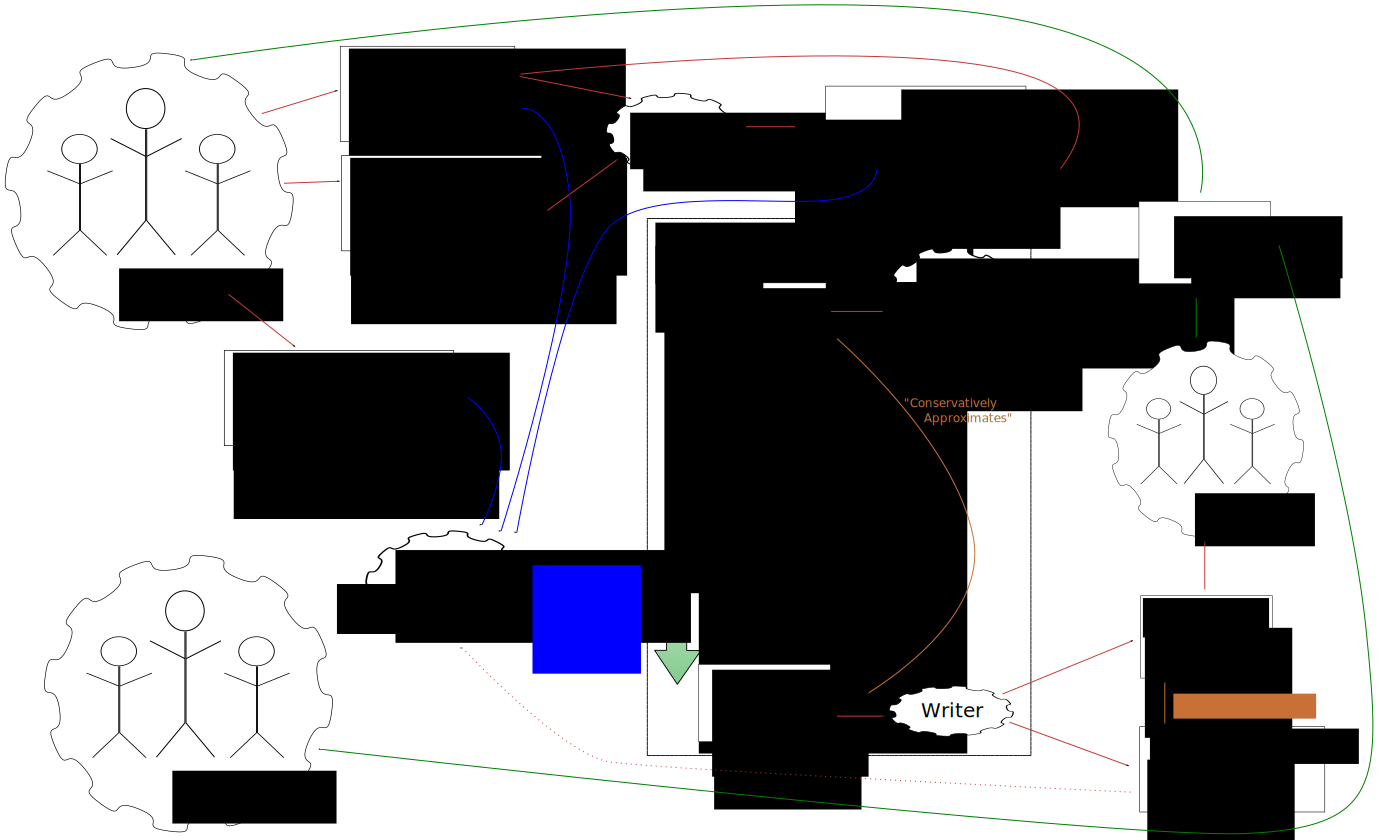
\includegraphics[width=12cm]{vl}
\end{center}
\end{frame}


\end{document}
